\documentclass{article}

%\usepackage{amsmath}
\usepackage{amsmath,amsfonts,amssymb,amsthm}
\usepackage{graphicx}
%\graphicspath{{fig/}}


\title{SIR model with shielded and isolated population}
\author{Req 550 Syria Team}

\newcommand{\ddt}{\frac{\textrm{d}}{\textrm{d}t}}

\begin{document}

\maketitle 

\section{Model}

\begin{align}
    \dot{S} &= - \frac{\beta}{N} E S + \alpha*N -\mu S,\label{eqn:basicSEIR_S}\\
    \dot{S_S} &= - \frac{\beta_{S}}{N} E_S S_S -\frac{\beta_{S,ext}}{N} E S_S,\label{eqn:basicSEIR_SS}\\
    \dot{E} &=+ \frac{\beta}{N} E S-\gamma_{E}E - \mu E,\label{eqn:basicSEIR_E}\\
    \dot{E_S} &=+ \frac{\beta_{S}}{N} E_S S_S
                 +\frac{\beta_{S,ext}}{N} E S_S -\gamma_{E}E_S-\mu E_S,
                 \label{eqn:basicSEIR_ES}\\
    \dot{I} &= +\gamma_{E}(E+E_S)-\gamma_{I} I - \mu I, \label{eqn:basicSEIR_I}\\
    \dot{R} &= \gamma_{I} I - \mu R. \label{eqn:basicSEIR_R}
\end{align}

\begin{figure}[ht]
    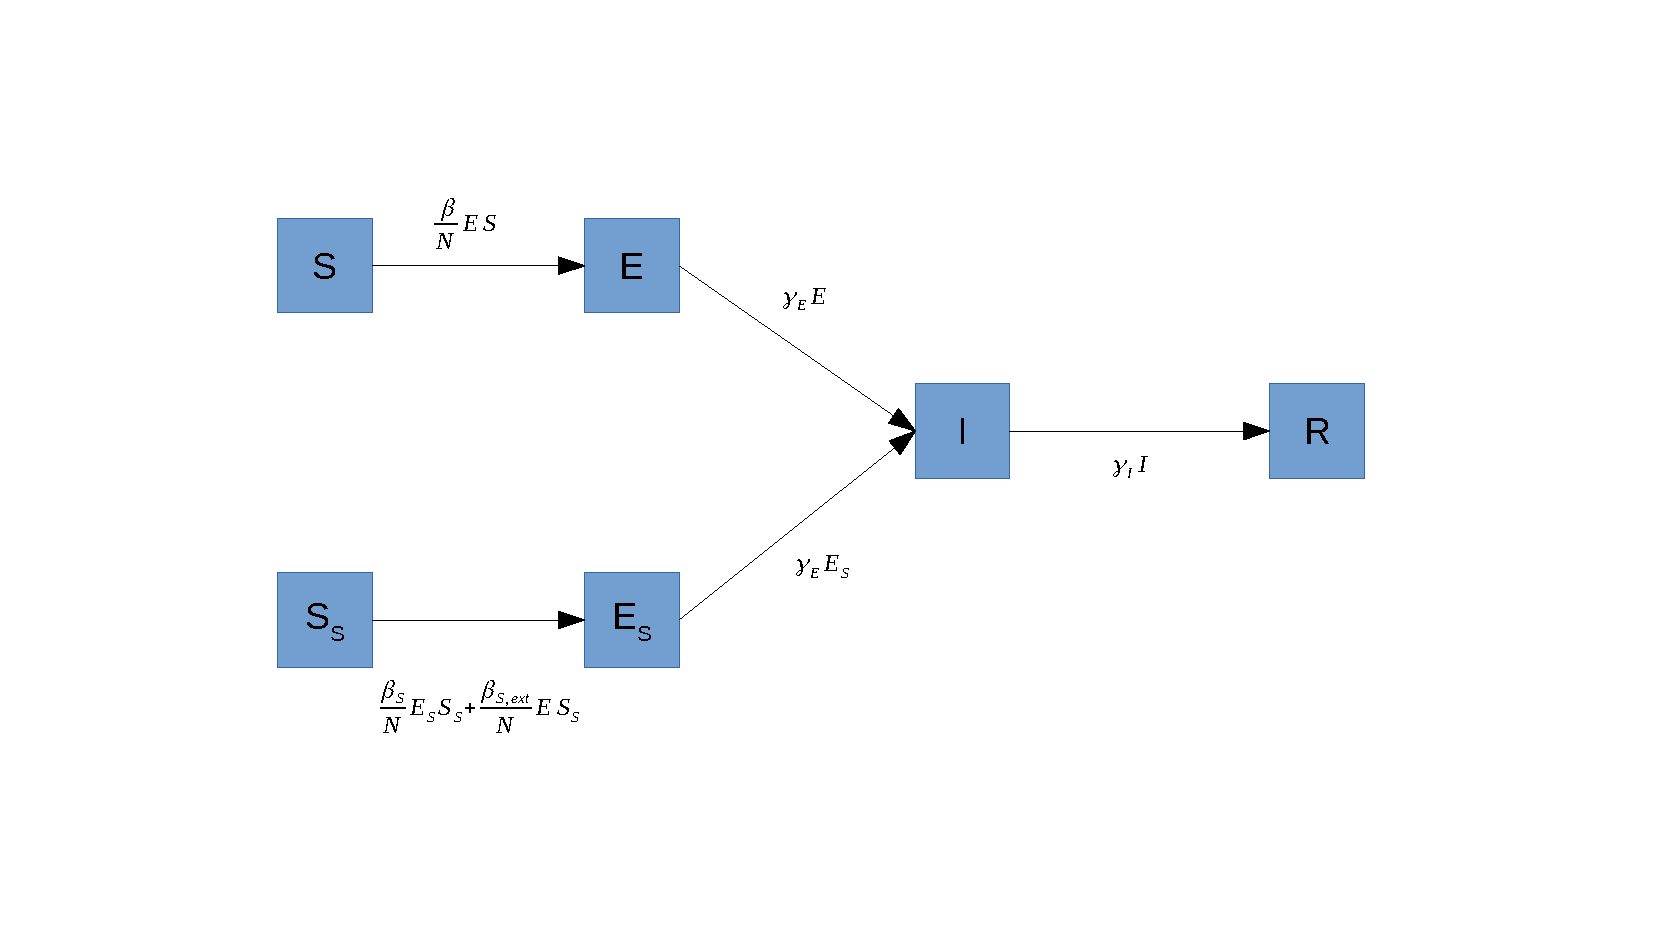
\includegraphics[width=.95\linewidth]{seir_shielded_diagram}
    \caption{Flow chart of the model.}\label{fig:seir_diagram}
\end{figure}


\section{Notation}

In the model, $S$ represents the population susceptible to be infected by the
disease. $E$ represents undetected infectious individuals (note that this
differs from other models where $E$ models exposed non-infectious). The
subscript $S$ distinguishes the general population and the shielded population.
Finally, $I$ is the number of detected cases, and $R$ the number of individuals
that had the disease (in the present formulation, this includes recovered and
death). See Figure \ref{fig:seir_diagram} for an schematic representation of
the model.

\section{Parameters}

The parameter $\beta$ controls the interaction between individuals. Similarly
$\beta_S$ controls the interaction between individuals within the shielded
population, whilst $\beta_{S,ext}$ controls the interaction between the
shielded population and the rest of the camp. $\gamma_E$ is (one over) the
average time to detect infectious individuals. $\gamma_I$ is (one over) the
average time from detection to recovery.

The birth rate $\alpha$ is included only in the general population. Natural
(non COVID related) death rate $\mu$ is included in all compartments.


\section{Rationale}

We want to model the dynamics of two interacting populations, the general
population of the camp, and the shielded population. We make the following
assumptions:

\begin{enumerate}
\item The two populations are well mixed (i.e., within each population,
everybody interacts with everybody).
\item The confirmed cases ($I$) are isolated from the rest of the population.
\item The shielded population has limited contact with the infectious
individuals in the general population ($\beta_{S,ext}$). 
\end{enumerate}

\section{Example}

Consider a camp with a population of 2000, and assume 10\% of the population
will be shielded. Assume that initially there is 1 infected individual in the
general population. 

Assuming that infected are detected as soon as they exhibit symptoms, we
consider $\gamma_E = 0.1$ (10 days) and $\gamma_I = 0.1$. Note that this values
can be estimated more accurately, but they are of the right order. 

Assume $\beta = \beta_S = 0.5$, based on the estimates for the Rohingya camps,
and assuming that within the shielded population individuals interact freely.
We take $\beta_{S,ext} = \beta/10$, to account for the fact that approximately
10\% of the shielded population will have contact with the rest of the camp.

Birth and death rates are taken from the overall Syria rates, as estimated by
J. Villers.

With this parameters, the model exhibits the dynamics represented in Figure
\ref{fig:seir_solution}. Note that after about 100 days the solution is mostly
stable and the shielded population remains constant and uninfected but in this
scenario most of the general population will have the disease at the same time.

\begin{figure}[ht]
    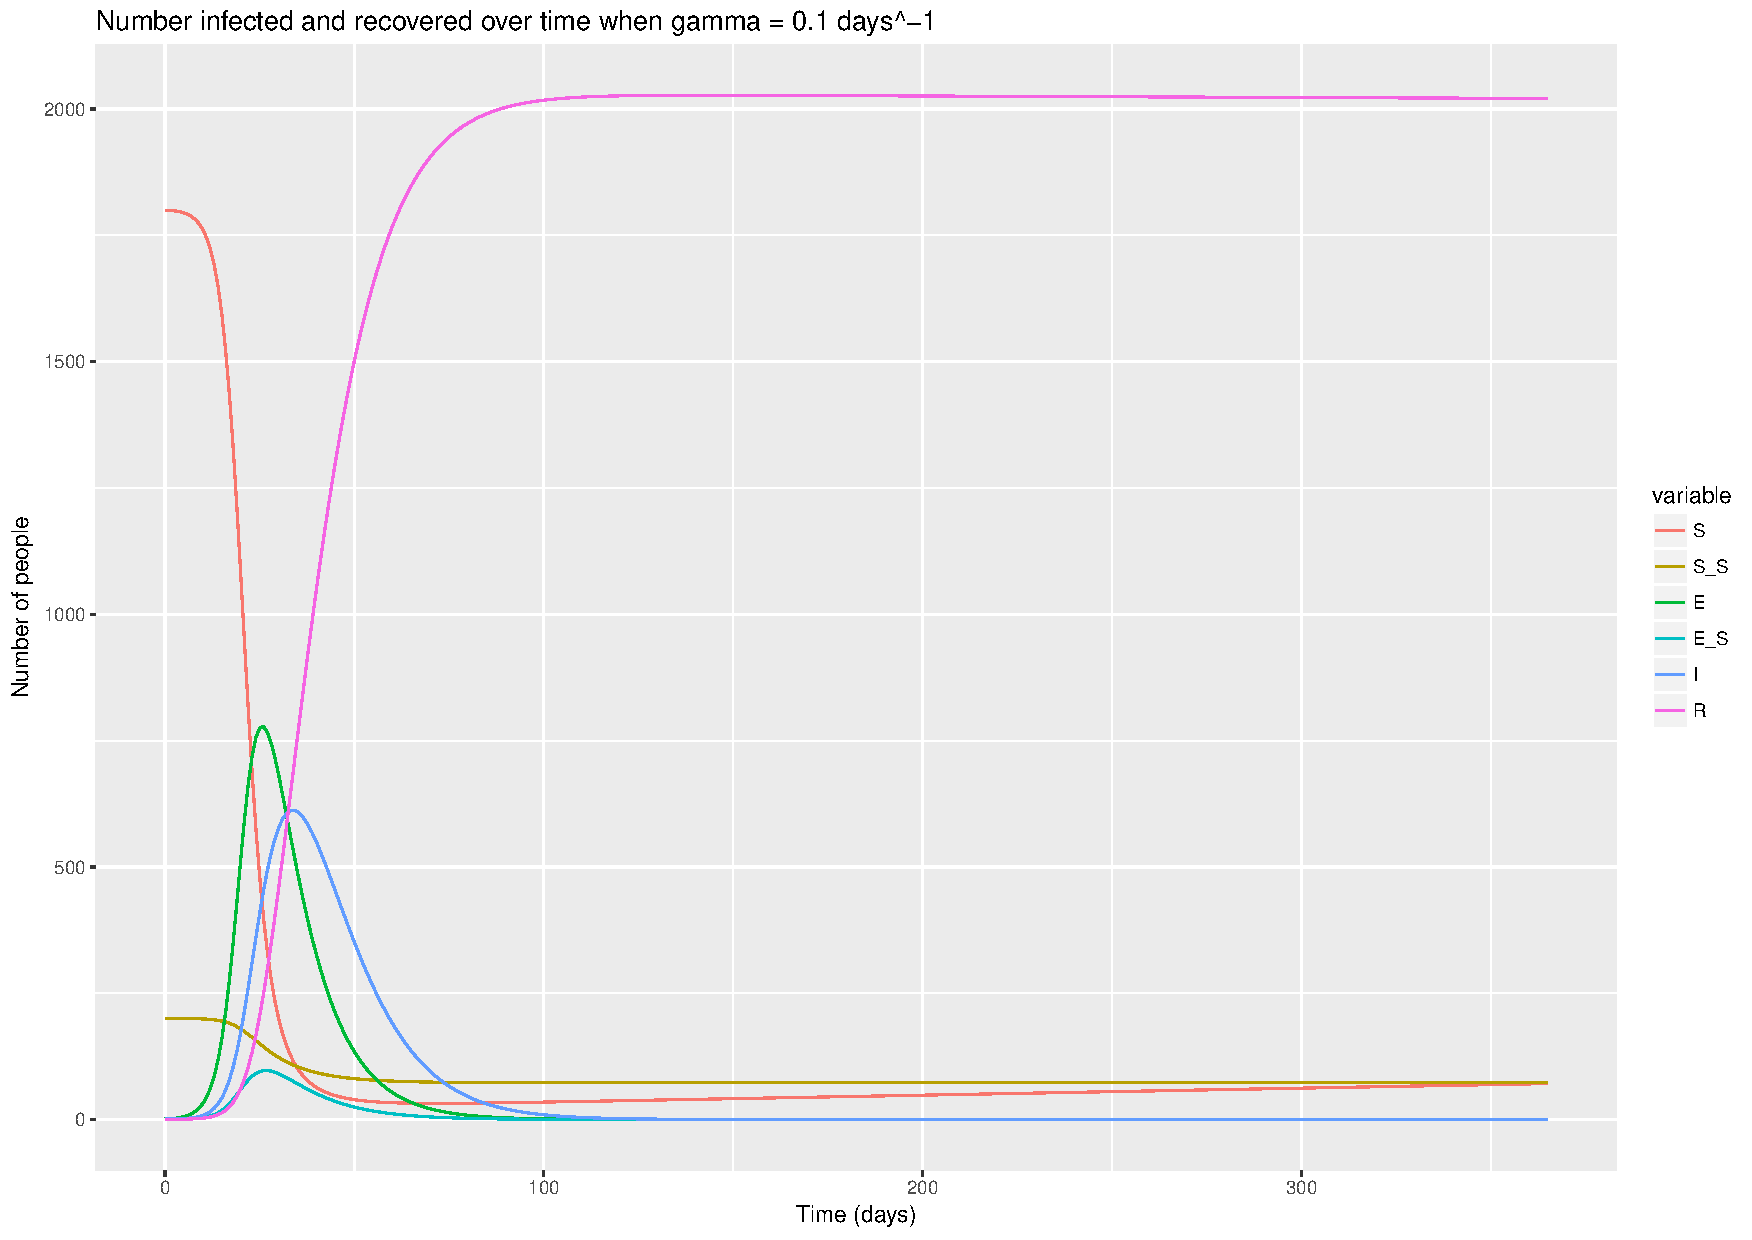
\includegraphics[width=.95\linewidth]{seir_solution}
    \caption{Solution with parameters described in the
text.}\label{fig:seir_solution}
\end{figure}

\section{TO DO}

To avoid double counting deaths, we have to split the R compartment to
distinguish deaths from recovered individuals.

Natural death rate in shielded population, flux of individuals from
general to shielded pop.

Account for asymptomatic individuals, that will remain infectious and in
contact with the population. Fraction of asymptomatic cases can be estimated
from other countries.


\end{document}
